\section{Auswertung}
\label{sec:Auswertung}
In der folgenden Tabelle sind alle Messwerte aufgeführt.
\begin{table}
  \centering
  \begin{tabular}{c c c c c c}
    \toprule
    Zeit/min & $T_1/\si{\kelvin}$ & $T_2/\si{\kelvin}$ & $p_a/\si{\bar}$ & $p_b/\si{\bar}$ & $N/\si{\watt}$ \\
    \midrule
    0 & 294.8\pm0.1 & 295.0\pm0.1 &  5.1\pm0.1 &  5.2\pm0.1  & 170\pm5 \\
    1 & 295.2\pm0.1 & 294.9\pm0.1 &  2.4\pm0.1 &  7.0\pm0.1  & 170\pm5 \\
    2 & 296.4\pm0.1 & 294.9\pm0.1 &  2.8\pm0.1 &  7.2\pm0.1  & 180\pm5 \\
    3 & 297.7\pm0.1 & 294.0\pm0.1 &  3.0\pm0.1 &  7.7\pm0.1  & 190\pm5 \\
    4 & 299.3\pm0.1 & 292.5\pm0.1 &  3.1\pm0.1 &  8.2\pm0.1  & 195\pm5 \\
    5 & 301.1\pm0.1 & 290.7\pm0.1 &  3.1\pm0.1 &  8.3\pm0.1  & 200\pm5 \\
    6 & 303.0\pm0.1 & 288.9\pm0.1 &  3.1\pm0.1 &  9.0\pm0.1  & 200\pm5 \\
    7 & 305.1\pm0.1 & 287.2\pm0.1 &  3.1\pm0.1 & 10.0\pm0.1  & 205\pm5 \\
    8 & 308.2\pm0.1 & 285.4\pm0.1 &  3.1\pm0.1 & 10.5\pm0.1  & 205\pm5 \\
    9 & 310.6\pm0.1 & 283.8\pm0.1 &  3.1\pm0.1 & 10.9\pm0.1  & 208\pm5 \\
   10 & 310.0\pm0.1 & 282.1\pm0.1 &  3.1\pm0.1 & 10.4\pm0.1  & 210\pm5 \\
   11 & 311.9\pm0.1 & 280.5\pm0.1 &  3.1\pm0.1 & 11.7\pm0.1  & 208\pm5 \\
   12 & 313.5\pm0.1 & 279.1\pm0.1 &  3.1\pm0.1 & 11.0\pm0.1  & 208\pm5 \\
   13 & 315.2\pm0.1 & 277.5\pm0.1 &  3.1\pm0.1 & 11.4\pm0.1  & 210\pm5 \\
   14 & 316.7\pm0.1 & 276.1\pm0.1 &  3.1\pm0.1 & 11.9\pm0.1  & 210\pm5 \\
   15 & 318.3\pm0.1 & 274.7\pm0.1 &  3.2\pm0.1 & 12.0\pm0.1  & 210\pm5 \\
   16 & 319.8\pm0.1 & 273.6\pm0.1 &  3.2\pm0.1 & 12.5\pm0.1  & 210\pm5 \\
   17 & 321.1\pm0.1 & 272.8\pm0.1 &  3.2\pm0.1 & 13.0\pm0.1  & 210\pm5 \\
   18 & 322.6\pm0.1 & 272.4\pm0.1 &  3.2\pm0.1 & 13.1\pm0.1  & 210\pm5 \\
   19 & 323.8\pm0.1 & 272.1\pm0.1 &  3.2\pm0.1 & 13.5\pm0.1  & 210\pm5 \\
   \bottomrule
  \end{tabular}
  \caption{Messdatentabelle.}
  \label{tab:Data}
\end{table}

Die Temperaturverläufe sind in dem folgenden Diagramm dargestellt und mit einer
linearen Ausgleichstrechnung approximiert.
\subsection{Temperaturausgleichskurve}
\begin{figure}
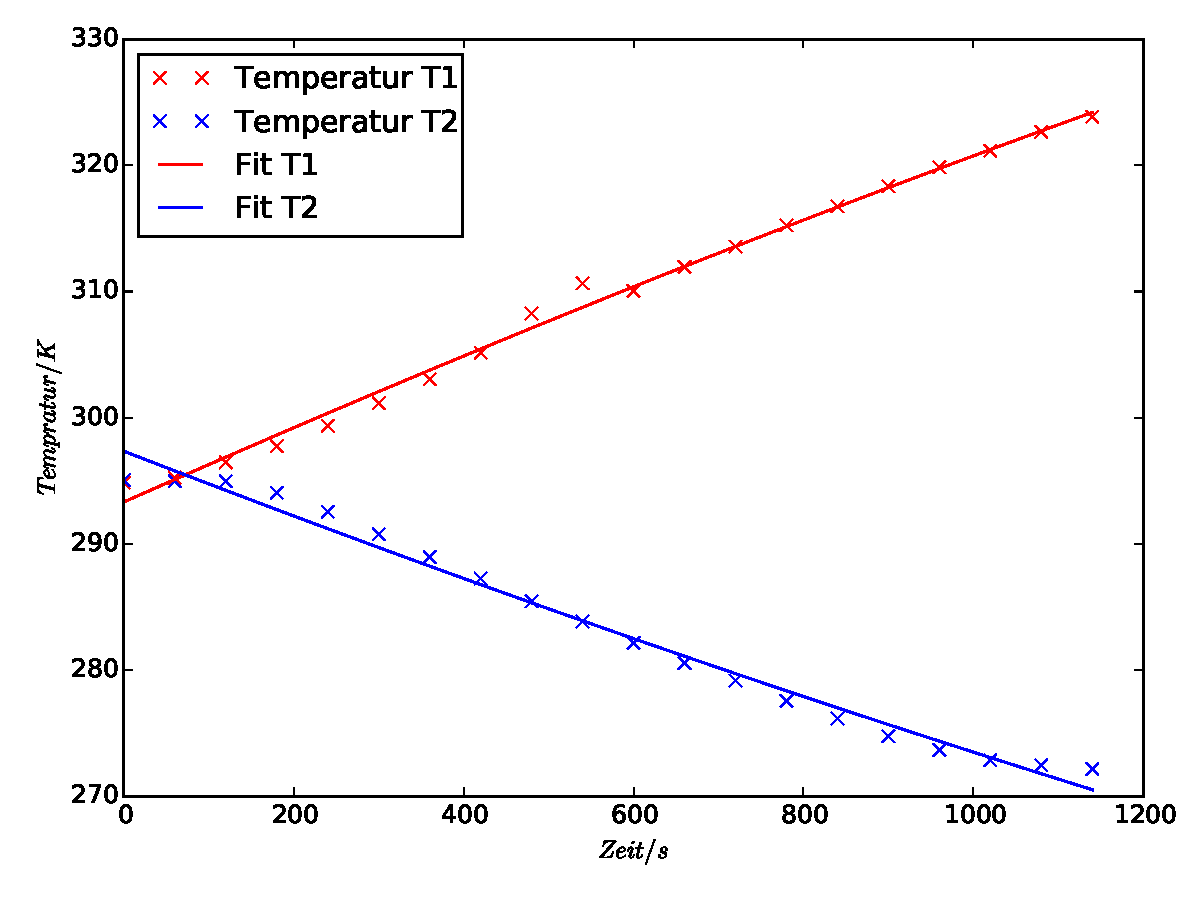
\includegraphics[height=13cm]{Temperaturgraphik.pdf}
\caption{Temperturausgleichskurve.}
\end{figure}

Die Näherung wurde mit scientific Python gemacht und ist gegeben durch
\begin{equation}
  T(t)=At^2+Bt+C .
\end{equation}
Die Parameter für erwärmte Reservoir $T_1$ sind

  $A=(-0.000002485)\si{\frac{\kelvin}{\sekunden^2}}$

  $B=(0.029925168)\si{\frac{\kelvin}{\sekunden}}$

  $C=(293.312793014)\si{\kelvin}$

Die Parameter für den anderen Behälter $T_2$ sind

  $A=(0.000002259)\si{\frac{\kelvin}{\sekunden^2}}$

  $B=(-0.026112097)\si{\frac{\kelvin}{\sekunden}}$

  $C=(297.339350549)\si{\kelvin}$$

Die dazugehörigen Differentialquotienten erhält man durch die folgende Gleichung
\begin{equation}
\frac{dT}{dt}=2At+B
\end{equation}

\begin{table}
  \centering
  \begin{tabular}{c c c}
    \toprule
    $Zeit/s$ & $dT_1 /dt$ & $dT_2 /dt$ \\
    \midrule
    300  &  0.028 & -0.024  \\
    600  &  0.027 & -0.023  \\
    900  &  0.025 & -0.022  \\
   1140  &  0.024 & -0.020  \\
   \bottomrule
 \end{tabular}
 \caption{Differentialquotienten.}
 \label{tab:Diffquo}
\end{table}
\subsection{Güteziffer}
Als nächstes soll die Güteziffer bestimmt werden dafür Nutzt man die Gleichung
\eqref{eqn:gueteziffer_ideal} für die ideale Güteziffer und die Gleichung
\eqref{eqn:gueteziffer_real}
\begin{table}
  \centering

  \begin{tabular}{c c c}
    \toprule
    $Zeit/s$ & $v_\symup{ideal}$ &  $v_\symup{real}$ \\
    \midrule
      300  &  28.956  &  1.875 \\
      600  &  11.112  &  1.692 \\
      900  &  7.301  &  1.598 \\
     1140  &  6.264  &  1.523 \\
   \bottomrule
 \end{tabular}
 \caption{Güteziffer}
 \label{tab:Gütez}
\end{table}
\subsection{Massendurchsatz}
Wenn man die Werte in Gleichung \eqref{eqn:massendurchsatz} einsetzt erhält man
den Massendurchsatz.
\begin{table}
  \centering
\begin{tabular}{c c c}
  \toprule
  $Zeit /s$ & $\frac{dQ_2}{dt}$ & $\frac{dm}{dt} /\frac{mol}{s}$  \\
  \midrule
  300  &   -326.430  & -0.014  \\
  600  &   -308.554  & -0.013  \\
  900  &   -290.679  & -0.012  \\
 1140  &   -276.379  & -0.012  \\
 \bottomrule
\end{tabular}
\caption{Massendurchsatz}
\label{tab:Massend}
\end{table}
\subsection{Mechanischekompressorleistung}
Die Dichte $\rho$, die für die Berechnung mechanischen Kompressorleistung
benötigt wird, kann berechnet werden, indem man die Gleichung der idealen Gase
umstellt.
\begin{equation}
  pV=nRT \leftrightarrow \frac{pV}{T}=nR
\end{equation}
Damit ergibt sich, da die Stoffmenge $n$ konstant bleibt,
\begin{equation}
  n_1=n_2
  \frac{p_0 V_0}{T_0}=\frac{p_2 V_2}{T_2}
\end{equation}
Da $ \rho V=m$ \leftrightarrow $V= \frac{m}{\rho}$ lässt sich \rho bestimmen wobei
$\rho_2=\rho$ und $p_2=p_a$.
\begin{equation}
  \rho=\frac{\rho_0 T_0 p_a}{T_2 p_0}
\end{equation}
Und mit Gleichung \eqref{eqn:kompressorleistung}
\begin{equation}
N_\symup{mech}=\frac{1}{\kappa-1}\left(p_b \sqrt[\kappa]{\frac{p_a}{p_b}}-p_a\right)\frac{1}{\frac{\rho_0 T_0 p_a}{T_2 p_0}}\frac{dm}{dt}
\end{equation}

\begin{table}
  \centering
\begin{tabular}{c c c}
  \toprule
  $Zeit /s$ & Dichte$\rho/\frac{g}{m^3}$ & Leistung$N_\symup{mech} /W$  \\
  \midrule
  300  &   15.49  &  -0.0026 \\
  600  &   15.05  &  -0.0031 \\
  900  &   15.13  &  -0.0033 \\
 1140  &   21.65  &  -0.0024 \\
 \bottomrule
\end{tabular}
\caption{Massendurchsatz}
\label{tab:Massend}
\end{table}
